\documentclass{article}
\usepackage[utf8]{inputenc}
\usepackage[portuges]{babel}
\usepackage{csquotes}
\usepackage{geometry}
\usepackage[pdftex]{hyperref}
\usepackage{indentfirst}
\usepackage{amsthm}
\usepackage{amssymb}
\usepackage{amsmath}
\usepackage{mathrsfs}
\usepackage{graphicx}
\usepackage{float}

\newtheorem{definition}{Definição}
\newtheorem{theorem}{Teorema}
\newtheorem{lemma}[theorem]{Lema}
\newtheorem{example}{Exemplo}

\usepackage[backend = biber]{biblatex}
\addbibresource{segundo_trabalho.bib}

\geometry{left = 3cm, top = 3cm, bottom = 2cm, right = 2cm}

\title{Inferência Estatística \\ 2º Trabalho}
\author{Igor Patrício Michels}
\date{16/09/2020}

\begin{document}

\maketitle

\section*{Introdução}

Trabalho elaborado pelo aluno Igor Patrício Michels referente a disciplina de Inferência Estatística, do quarto período da Graduação em Matemática Aplicada da FGV-EMAp. Nele discutiremos o Algoritmo EM, além de visitarmos um exemplo de sua aplicação.

O enunciado e eventuais funções utilizadas para resolução deste ou de outros trabalhos podem ser encontrados \href{https://github.com/IgorMichels/Statistical_Inference}{\textbf{nesse repositório do GitHub}}.

\section*{O Algoritmo EM}

\subsection*{O Algoritmo EM}

O Algoritmo EM é um algoritmo iterativo que visa estimar a máxima verossimilhança quando os dados obtidos são incompletos. Historicamente, esse algoritmo foi explicado por Dempster, Laird e Rubin (veja \cite{10.2307/2984875}), entretanto com uma análise de convergência falha. Em 1983, Wu faz um novo estudo sobre o algoritmo e nele apresenta uma análise correta para a convergência do algoritmo (veja \cite{wu1983}).

Feita uma breve apresentação histórica, podemos definir o Algoritmo EM de forma similar a Wu (em \cite{wu1983}) e Casella (em \cite{casella}).

Tomamos dois conjuntos $\mathscr{X}$ e $\mathscr{Y}$ onde $\mathscr{X}$ representa o conjunto de dados faltantes e $\mathscr{Y}$ representa o conjunto de dados observados, assim podemos estabelecer uma relação de muitos para um entre $\mathscr{X}$ e $\mathscr{Y}$\footnote{Note que essa relação existe em virtude de que os dados faltantes podem ser qualquer um dentre os possíveis.}. Agora, seja $\theta$ o vetor de parâmetros a serem estimados, $\theta^{(p)}$ a estimativa na $p$-ésima iteração do algoritmo, seja também $x \in \mathscr{X}$ um conjunto de dados faltantes, um conjunto de dados observados $y \in \mathscr{Y}$ e de forma que $(y, x)$ representa o dado completo. Assim, $f(y, x | \theta)$ é a função de densidade de probabilidade dos dados completos com parâmetros $\theta \in \Omega$ e a função de densidade de probabilidade de $y$ dada por $g(y | \theta)$ de forma que
\[g(y | \theta) = \int f(y, x | \theta) ~dx.\]

Agora, note que o parâmetro $\theta$ é estimado pelo método da máxima verossimilhança dos dados observados, ou seja, maximizando $L(\theta | y)$, que é a função de verossimilhança dos dados observados. Nesse ponto, podemos fazer algumas observações:
\begin{enumerate}
    \item
        a função de verossimilhança dos dados completos é a função $L(\theta | y, x) = f(y, x | \theta)$;
        
    \item
        maximizar uma função é equivalente a maximizar o logaritmo da mesma função, assim, por simplicidade, pode ser interessante trabalhar com a função de log-verossimilhança;
        
    \item
        em geral, o mais simples é maximizar a função com os dados completos, ou seja, maximizar $L(\theta | y, x)$ é, em geral, mais simples que maximizar $L(\theta | y)$.
\end{enumerate}

Feitas tais observações, iremos pensar em maximizar a função de log-verossimilhança. Para tanto, definimos uma nova função
\[k(x | \theta, y) = \dfrac{f(y, x | \theta)}{g(y | \theta)}\]

\noindent a qual é a densidade condicional de $x$ dados $y$ e $\theta$. Assim, podemos reescrever
\[g(y | \theta) = \dfrac{f(y, x | \theta)}{k(x | \theta, y)},\]

\noindent o que nos dá
\[\log{L(\theta | y)} = \log{L(\theta | y, x)} - \log{k(x | \theta, y)}.\]

Entretanto, note que $x$ não foi observado, então podemos substituir o lado direito da equação acima elo valor esperado de $k(x | \theta^{(0)}, y)$, nos dando

\[\log{L(\theta | y)} = E\left[\log{L(\theta | y, X)} | \theta^{(0)}, y\right] - E\left[\log{k(X | \theta, y)} | \theta^{(0)}, y\right].\]

Agora, definido $\theta^{(0)}$, podemos iterar o Algoritmo EM da seguinte forma:
\begin{itemize}
    \item
        {\textbf{E-step}} determine o valor esperado da função de log-verossimilhança dos dados: $E\left[\log{L(\theta | y, x)} | \theta^{(p)}, y\right]$;
        
    \item
        {\textbf{M-step}} escolha $\theta^{(p + 1)}$ de forma a maximizar a função definida no passo anterior e, em seguida, tome $p = p + 1$.
\end{itemize}

Um outro detalhe muito importante do Algoritmo EM é que durante a execução do algoritmo obtemos uma sequência $\{\theta^{p}\}$ monotônica e não decrescente com respeito à verossimilhança, ou seja,
\[L\left(\theta^{(p + 1)} | y\right) \geq L\left(\theta^{(p)} | y\right).\]

Podemos enunciar e demonstrar esse teorema.

\begin{theorem}
    \label{teo}
    A sequência $\{\theta^{(p)}\}$ obtida durante a iteração do Algoritmo EM é tal que
    \[L\left(\theta^{(p + 1)} | y\right) \geq L\left(\theta^{(p)} | y\right).\]
\end{theorem}

\begin{proof}
    Primeiramente, perceba que o Algoritmo EM realiza um procedimento que visa maximizar a a função de log-verossimilhança e, consequentemente, a função de verossimilhança. O algoritmo funciona maximizando uma função $Q(\theta, \theta^{(p)})$, fácil de maximizar e que serve de limite inferior para $\log{L(\theta)}$, além disso, temos que $\log{L(\theta^{(p)})} = Q(\theta^{(p)}, \theta^{(p)})$. Entretanto, a cada iteração buscamos maximizar $Q$ com $\theta^{(p + 1)}$, logo, devemos ter que, ao maximizar $Q$, $Q\geq \log{L(\theta^{(p)})}$ e, como $Q$ atua como limite inferior de $\log{L(\theta)}$, teremos $\log{L(\theta^{(p + 1)})}\geq \log{L(\theta^{(p)})}$.
    
    De forma mais matemática:
    \begin{equation*}
        \begin{split}
            \log{L(\theta)} & = \sum \log{p(y_i | \theta)} \\
            & = \sum \log{\sum_x p(y_i, x | \theta)} \\
            & = \sum \log{\sum_x p\left(x | y_i, \theta^{(p)}\right)\cdot \dfrac{p(y_i, x | \theta)}{p\left(x | y_i, \theta^{(p)}\right)}} \\
            & \geq \sum \sum_x p\left(x | y_i, \theta^{(p)}\right)\cdot \dfrac{p(y_i, x | \theta)}{p\left(x | y_i, \theta^{(p)}\right)} \\
            & \equiv Q\left(\theta, \theta^{(p)}\right).
        \end{split}
    \end{equation*}
    
    Note que, ao incluir $p\left(x | y_i, \theta^{(p)}\right)$ estamos calculando de forma separadamente cada amostra $y_i$. Além disso, a desigualdade acima surge com a aplicação da Desigualdade de Jensen.
    
    Note também que
    \[Q\left(\theta^{(p)}, \theta^{(p)}\right) = \sum \log{p\left(y_i | \theta^{(p)}\right)} = \log{L\left(\theta^{(p)}\right)}.\]
    
    Agora, lembramos que durante a execução do passo M encontramos $\theta^{(p + 1)}$ de forma a maximizar $Q$, assim
    \[Q\left(\theta^{(p + 1)}, \theta^{(p)}\right) \geq Q\left(\theta^{(p)}, \theta^{(p)}\right) = \log{L\left(\theta^{(p)}\right)}\]
    
    \noindent e, usando que $Q$ é uma cota inferior para $\log{L}$, temos
    \[\log{L\left(\theta^{(p + 1)}\right)} \geq Q\left(\theta^{(p + 1)}, \theta^{(p)}\right) \geq Q\left(\theta^{(p)}, \theta^{(p)}\right) = \log{L\left(\theta^{(p)}\right)},\]
    
    \noindent o que implica em
    \[L\left(\theta^{(p + 1)}\right) \geq L\left(\theta^{(p)}\right).\]
\end{proof}

\subsection*{Uma aplicação do Algoritmo}

Uma vez que já fomos apresentados ao Algoritmo EM, podemos vê-lo em prática em um exemplo.

\begin{example}
    \label{example1}
    Suponha que temos duas moedas, Moeda 1 e Moeda 2 de modo que $Pr(\textit{Cara }|\textit{ Moeda} = 1) = p_1$ e $Pr(\textit{Cara }|\textit{ Moeda} = 2) = p_2$; Suponha que agora façamos o seguinte experimento:
    \begin{enumerate}
        \item[(i)]
            selecionamos uma moeda aleatoriamente com probabilidade $\frac{1}{2}$;
            
        \item[(ii)]
            lançamos a moeda selecionada $m$ vezes;
            
        \item[(iii)]
            repetimos (i) e (ii) $n$ vezes.
    \end{enumerate}
        
    Podemos representar os dados advindos desse experimento como
    \begin{equation*}
        \begin{array}{ccccc}
            X_{11} & \dots & X_{1m} & & M_1 \\
            X_{21} & \dots & X_{2m} & & M_2 \\
            \vdots & \ddots & \vdots & & \vdots \\
            X_{n1} & \dots & X_{nm} & & M_n 
        \end{array}
    \end{equation*}
    
    \noindent onde $X_{ij}$ é a variável de Bernoulli que representa o resultado do $j$-ésimo lançamento da moeda na $i$-ésima rodada e $M_i \in \{1, 2\}$ é a variável aleatória que guarda a informação sobre qual moeda foi lançada na $i$-ésima rodada do experimento.
    
    Desenvolva um esquema EM para obter o EMV de $\theta = (p_1, p_2)$ quando desconhecemos os valores de $M_i$, isto é, quando não sabemos que moeda foi escolhida em cada uma das $n$ rodadas.
\end{example}

Em nosso exemplo, temos apenas os $X$'s, ou seja, dispomos apenas de
\begin{equation*}
    \begin{array}{ccc}
        X_{11} & \dots & X_{1m} \\
        X_{21} & \dots & X_{2m} \\
        \vdots & \ddots & \vdots \\
        X_{n1} & \dots & X_{nm} 
    \end{array}
\end{equation*}

\noindent e queremos fazer uma estimativa de $\theta = (p_1, p_2)$. Note que se tivéssemos os $M$'s seria muito simples de fazer a estimativa de $\theta$, bastava separar os dados que representam $M = 1$ e os dados em que temos $M = 2$ e calcular $p_1$ e $p_2$ separadamente. Entretanto, como não temos os $M$'s, vamos utilizar o algoritmo que acabamos de ver.

Para utilizar o Algoritmo EM, vamos definir que $X_{ij} \in \{0, 1\}$, sendo que $X_{ij} = 1$ representa que o $j$-ésimo lançamento da moeda na $i$-ésima rodada resultou em cara e $X_{ij} = 0$ irá representar que tal lançamento resultou em coroa.

Agora, seguindo a ideia descrita pelo algoritmo EM, vamos considerar $\theta^{(0)} = \left(\frac{1}{2}, \frac{1}{2}\right)$.\footnote{Aqui também poderíamos tomar $\theta^{(0)} = \left(p_1^{(0)}, p_2^{(0)}\right)$ qualquer, uma vez que iremos atualizar o valor de $\theta$ durante as iterações.} Feito isso, podemos ir para o passo E, ou seja, vamos escrever a função de log-verossimilhança

\begin{equation*}
    \begin{split}
        Q\left(\theta | \theta^{(0)}\right) & = \ln{\left(\prod_{i = 1}^{n} \left(\dfrac{1}{2}\prod_{j = 1}^{m} Pr\left(X_{ij} = x_{ij} | M_i = 1\right) + \dfrac{1}{2}\prod_{j = 1}^{m} Pr\left(X_{ij} = x_{ij} | M_i = 2\right)\right)\right)} \\
        & = \sum_{i = 1}^{n} \ln{\left(\frac{1}{2}\prod_{j = 1}^{m} Pr(X_{ij} = x_{ij} | M_i = 1) + \frac{1}{2}\prod_{j = 1}^{m} Pr(X_{ij} = x_{ij} | M_i = 2)\right)}
    \end{split}
\end{equation*}

\noindent onde $Pr\left(X_{ij} = x_{ij} | \theta^{(0)}, M_i = 1\right) = \frac{1}{2}$ se $x_{ij} = 1$ e $Pr\left(X_{ij} = x_{ij} | \theta^{(0)}, M_i = 1\right) = \frac{1}{2}$ se $x_{ij} = 0$. Analogamente, $Pr\left(X_{ij} = x_{ij} | \theta^{(0)}, M_i = 2\right) = \frac{1}{2}$ se $x_{ij} = 1$ e $Pr\left(X_{ij} = x_{ij} | \theta^{(0)}, M_i = 2\right) = \frac{1}{2}$ se $x_{ij} = 0$.\footnote{No caso geral, vale que $Pr\left(X_{ij} = x_{ij} | \theta^{(0)}, M_i = 1\right) = p_1$ se $x_{ij} = 1$ e $Pr\left(X_{ij} = x_{ij} | \theta^{(0)}, M_i = 1\right) = 1 - p_1$ se $x_{ij} = 0$ e, de forma análoga, $Pr\left(X_{ij} = x_{ij} | \theta^{(0)}, M_i = 2\right) = p_2$ se $x_{ij} = 1$ e $Pr\left(X_{ij} = x_{ij} | \theta^{(0)}, M_i = 2\right) = 1 - p_2$ se $x_{ij} = 0$.}

Definida a função de log-verossimilhança podemos ir para o passo M: encontrar $\theta^{(1)}$ de forma que $\theta^{(1)}$ maximize $Q\left(\theta | \theta^{(0)}\right)$.

Feito isso, finalizamos a primeira iteração e podemos ficar repetindo esse processo.

Para ilustrar esse exemplo, coloquei no repositório do GitHub, um script ``Simulação Moedas.py''\footnote{Executei o script no VS Code utilizando Python 3.8.0.}, o qual faz a simulação do Exemplo \ref{example1} com os resultados da estimativa de $\theta$ para atribuições distintas de $\theta^{(0)}$.

No script, o usuário pode definir os parâmetros $\theta$, $m$ e $n$, a partir dos quais cria-se uma amostra aleatória de ``lançamentos de moedas''. Em seguida, podemos fazer a estimativa de $\theta$ da amostra gerada, basta dar um valor inicial para $\theta$ (definir um $\theta^{(0)}$) que as funções lá definidas irão retornar o valor estimado para $\theta$, bem como o valor da função de log-verossimilhança negativa.\footnote{Em python, utilizando a biblioteca scipy.optimize, podemos utilizar a função minimize, a qual irá buscar o valor mínimo de uma função já definida, dessa forma, se queremos maximizar a função de log-verossimilhança, podemos minimizar a função de log-verossimilhança negativa.}

\begin{figure}[H]
    \centering
    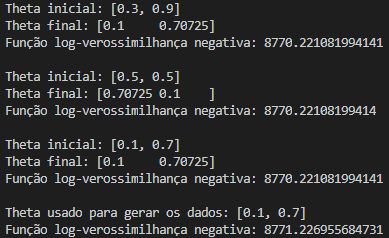
\includegraphics[scale = 0.7]{2º Trabalho/Script.png}
    \caption{Retorno do Scrip}
    \label{script}
\end{figure}

O script citado é uma ferramenta interessante para ilustrar o fato de que o algoritmo nem sempre irá nos levar a um máximo global da função de log-verossimilhança, mas a um máximo local. Além do script, o repositório do GitHub contém um Notebook\footnote{Para o Notebook, utilizei o Jupyter Notebook (Anaconda3), com o Python 3.} com a mesma simulação e com algumas informações sobre o desenvolvimento da simulação.

Uma outra aplicação do Algoritmo EM é dada na estimação de parâmetros para exames que utilizam a TRI - Teoria de Resposta ao Item. Para mais detalhes sobre essa aplicação veja \cite{IRT} ou então \cite{Rubin2001}.

\subsection*{Mais um pouco sobre o Algoritmo EM}

Conforme visto nas seções anteriores, o Algoritmo EM é um algoritmo iterativo que busca os parâmetros que irão maximizar a função de verossimilhança quando algumas variáveis não foram observadas e/ou coletadas. Além disso, o Teorema \ref{teo} nos afirma que a verossimilhança nunca diminui de uma iteração para outra, ou seja, conforme vamos aumentando o número de iterações, o valor da verossimilhança aumenta ou se mantém, assim, para uma sequência limitada $L(\theta^{(p)})$, isso significa que $L(\theta^{(p)})$ converge para um $L*$ (para mais detalhes, veja \cite{wu1983}).

Quanto a sua aplicabilidade, note que nem sempre os dados não coletados possuem relevância no problema, por exemplo, ao estimar a altura média de uma população não precisamos do nome dos indivíduos que observamos, entretanto é interessante observar o sexo dos mesmos para fazer uma estimativa separando os indivíduos pelo sexo. Dessa forma, se coletarmos apenas a altura do indivíduo e a proporção de homem e mulheres podemos estimar qual a altura média da população masculina e feminina.

Agora, embora o algoritmo se mostre um ferramental interessante, nem sempre é compensatório utilizá-lo, pois, mesmo em computadores com alto poder de processamento, suas iterações podem ficar lentas quando o volume de dados é muito grande e/ou quando a quantidade de dados faltantes é alta.\footnote{Note que, a cada iteração, buscamos o máximo de uma função que nem sempre é simples.} Além disso, pelo fato do Algoritmo EM nem sempre convergir para o valor de máxima verossimilhança, mas para um máximo local, pode ser interessante reaplicar o algoritmo diversas vezes com valores iniciais distintos para chegarmos, com maior probabilidade, no máximo global (\cite{statisticshowto}). Além disso, em muitos casos pode ser até mesmo mais simples utilizar um estimador de máxima verossimilhança, o qual apresentou resultados similares nas comparações realizadas por Stephen Walker em \cite{10.2307/2533054} ou então utilizar uma das variações do Algoritmo EM, as quais podem ser vistas brevemente em \cite{roche2011em}.

\section*{Conclusão}

Nesse trabalho vimos a definição do Algoritmo EM, bem como um exemplo de sua aplicação e uma breve análise do mesmo.

Conforme visto, o Algoritmo EM nos dá uma forma iterativa de calcular parâmetros para uma série de dados, mesmo que incompleta. Além disso, embora ocorra do algoritmo ficar lento, o mesmo não deixa de ser relevante, uma vez que o mesmo suporta séries de dados relativamente grandes dependendo do computador a ser utilizado e ainda ele é de fácil implementação computacional.

\printbibliography

\end{document}
